\chapter{Motivation for Planning-based Approach}

\label{Chapter3} % For referencing the chapter elsewhere, use \ref{Chapter1} 

A commonality of all of the previous algorithms is that they all use some degree of learning to try to determine the best actions to take at any given situation. However, this approach has some issues. For one, learning requires a large amount of training in order to generalize across the large state space. This is problematic, as the player data gathered over multiple sessions is relatively small. Additionally, because the agent only learns the best actions to take at the current time step, it lacks the ability to plan for a sequence of actions that form a cohesive strategy. This part is important, as individual playstyles are categorized by the strategies that a player tends to use. Lastly, there is a natural trade off between optimality and employing a degree of randomness when these agents decide the next action to take. If an AI always does the same action in response to a situation, it loses the unpredictability of human play. However, once an AI does a random action that is unreasonable for the current situation, players will instantly recognize it as an AI. 

\begin{figure}[h]
	\centering
	\begin{subfigure}[h]{0.4\textwidth}
		\centering
		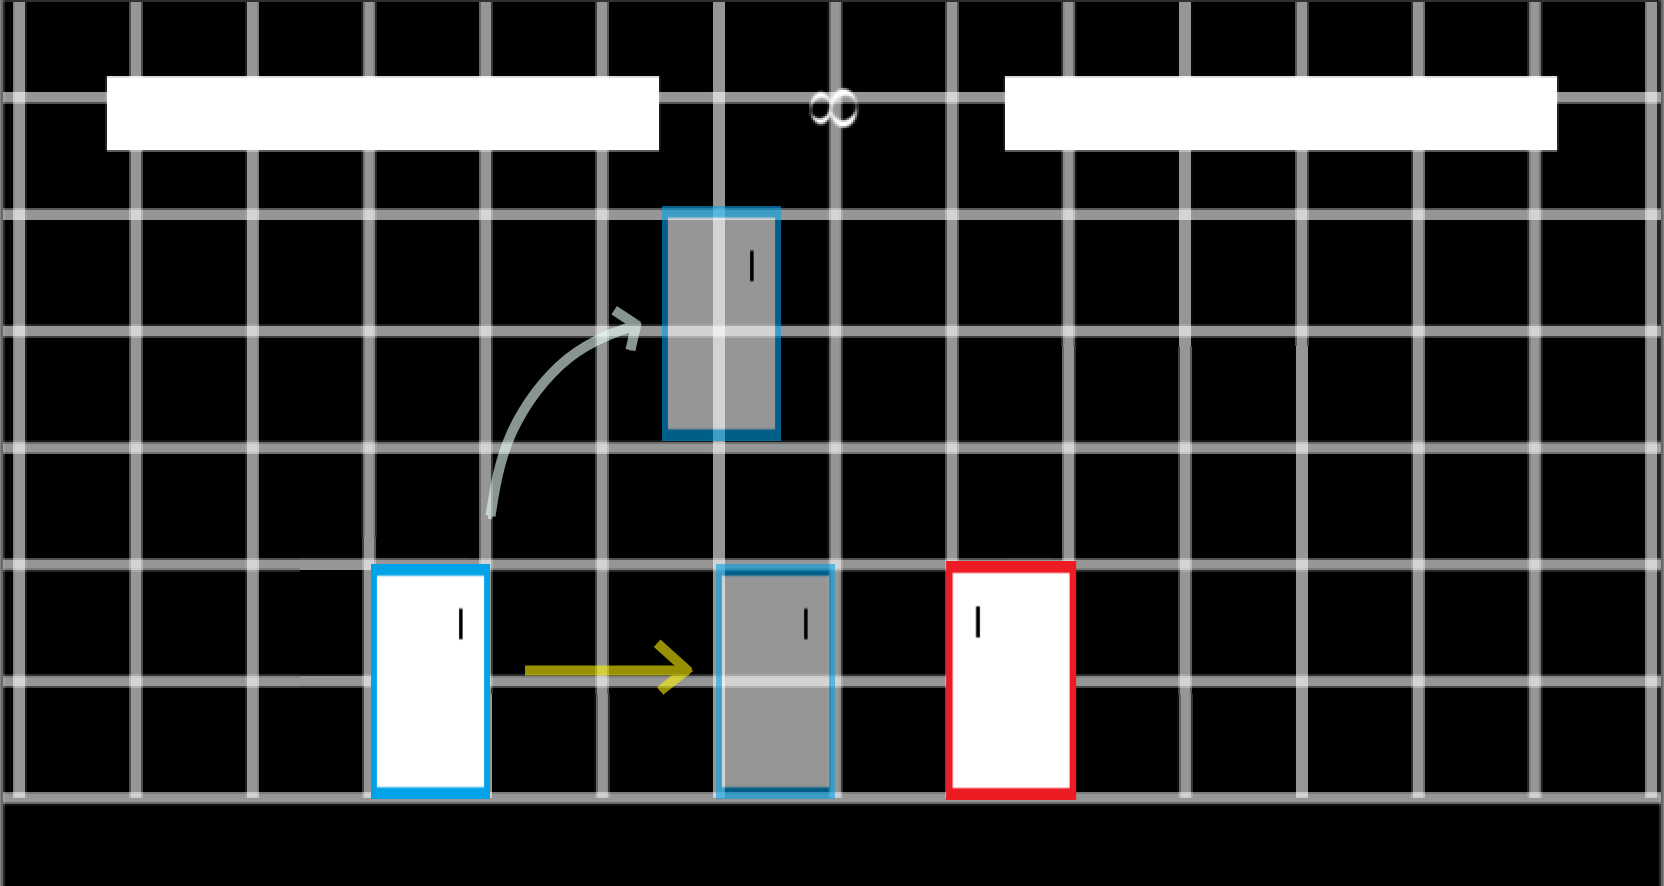
\includegraphics[width=\textwidth]{Figures/LearningExample1.png}
		\caption{A predictable AI is not very human-like}
		\label{Learning1}
	\end{subfigure}
	\begin{subfigure}[h]{0.4\textwidth}
		\centering
		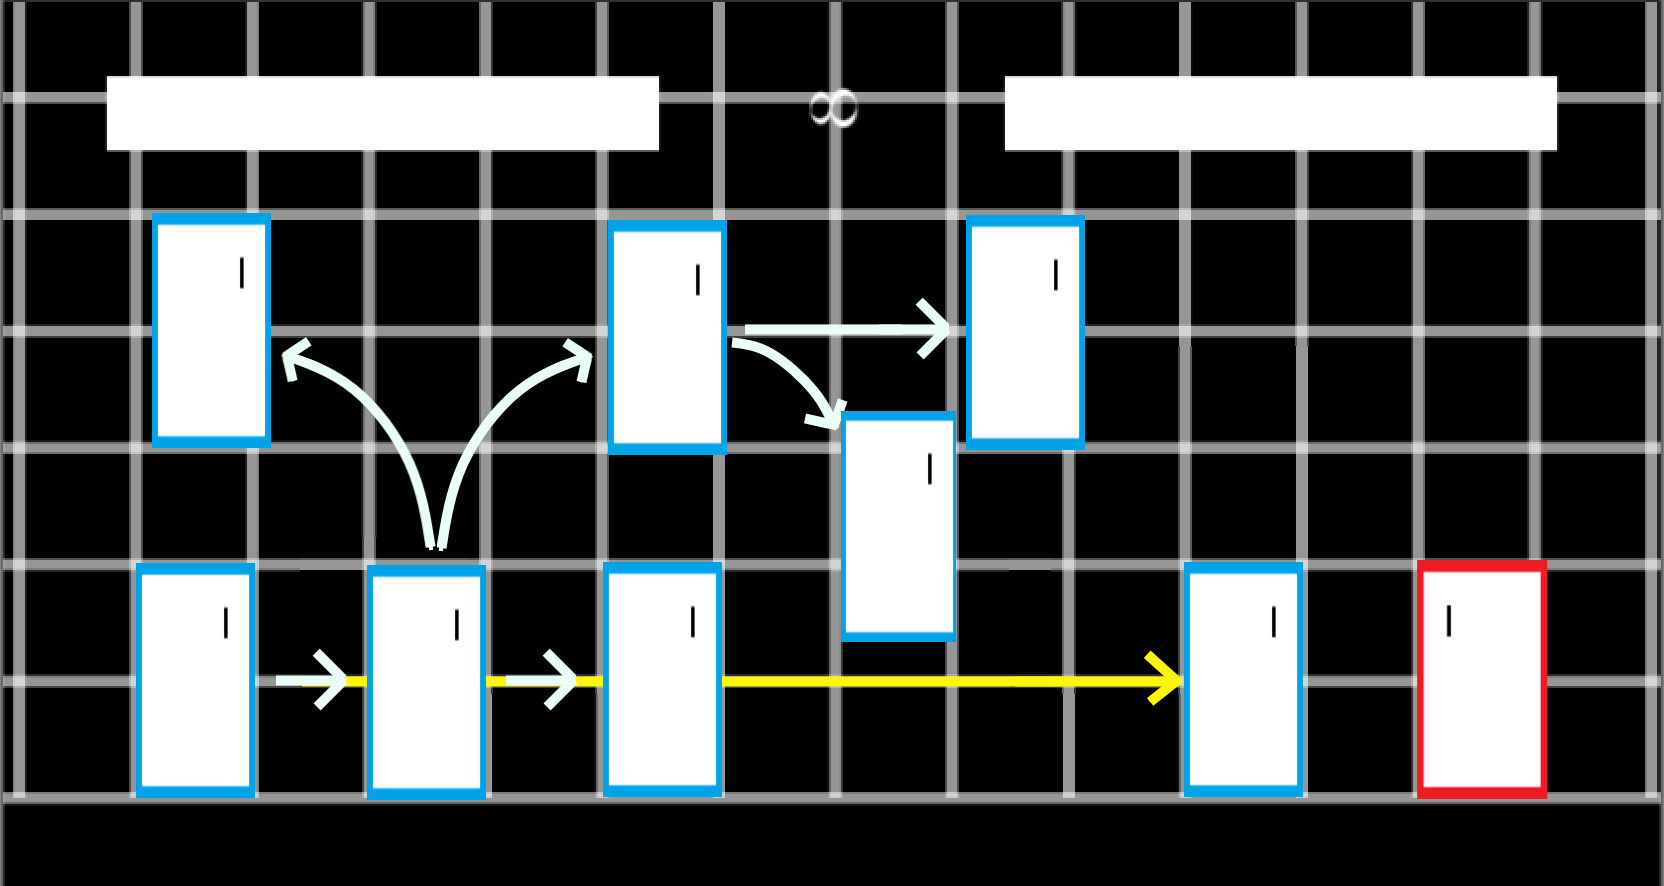
\includegraphics[width=\textwidth]{Figures/LearningExample2.png}
		\caption{One unreasonable action can break immersion}
		\label{Learning2}
	\end{subfigure}
\end{figure}

%This is because while learning techniques are very good at determining the right move to make given a situation, they don't do a great job at planning long-term strategies. 

%Even if the algorithm learns the distribution of the actions that the player tends to take, a chain of selections would still be unlikely to form something that resembles cohesive strategy. This is because the AI has to decide on an action to perform on every frame. This ultimately results in the jittery movements that characterizes these kinds of AI's in dynamic environments, as it's hard for it to decide to do a single action for a prolonged period of time.

\section{Why Use Search?}

Because human-play is heavily predicated on the usage of different kinds of strategies, dynamically creating and executing the same strategies as a target player should mimic their playstyle quite well. Since strategies are essentially a sequence of actions that a player takes in order to arrive at a desired goal, the formulation of strategies can naturally be represented as a search problem over the state space. The target player's demonstrations can be used to inform the AI of the goals to target and the actions to use, and custom heuristics can bias the search towards actions that closely mimic the player. In addition, the demonstrations can be used to create a model of the game state's dynamics, which would allow the AI to form cohesive plans even in unfamiliar starting states. 

To understand how an AI might effectively use search, consider the following situation:

\begin{figure}[h]
	\centering
	\includegraphics[width=\textwidth]{Figures/Flowchart.png}
	\caption{The target player's strategy}
	\label{Player Strategy}
\end{figure}

In the demonstration, player 1 tends to try to stay within a certain range of the opponent and try to hit them with a low attack. If the opponent blocks the low attack, it sometimes then tries to jump in while the opponent can't move out of the way and hit them with a air attack. Essentially, player 1's behavior is composed of 2 strategies, one where they try to hit the opponent with a low attack and another where they force the opponent to try to block the air attack. We can easily identify the strategy that the player is currently executing by looking at the ultimate result that they are aiming for.

%In a learning context, the AI has to decide at each frame what action it must do. This means that as the AI is walking towards the opponent, it must decide at each frame that the correct action to do is walk left. However, this results in a series of issues on the implementation side. First of all, it requires that we must record the players action during every frame of a training episode, as otherwise unknown states would pop up all of the time as the player moves forwards. Further more, we quickly find that the AI performs poorly when starting in an unfamiliar position. This is because it is unlikely to find its way to a state that it has properly been trained on, and because it tries to pick an action to do at every frame, it is unlikely to reach a stable state and settle back into a correct strategy. Though function approximators can alleviate the tendency of the AI to take essentially random moves, it still is fairly ineffective at predicting the proper action in states that are unlike anything it's trained on. Though the initial demonstration can give the AI a pretty good idea of what to do when presented the exact same situation, it quickly falls apart the second we reach an unknown state. Compounded with the fact that we want to represent the game state with several categorical variables, this approach will likely fail to be robust enough to represent a human AI.

When the AI plans, it first determines what goal state to target. It then uses the actions pulled from the target player's demonstration and uses them to search the state space to reach the goal. For example, to reach the goal where the opponent is hit with a low attack, the search would return a plan where it walks forward to get close to the opponent, crouches, and then uses the low attack. If the opponent moves during that time, the AI replans picks a walking action that would put it in the correct range for hitting the opponent. With a single demonstration, search is able to formulate a plan that approximately resembles the strategy executed by the target player.

\begin{figure}[h]
	\centering
	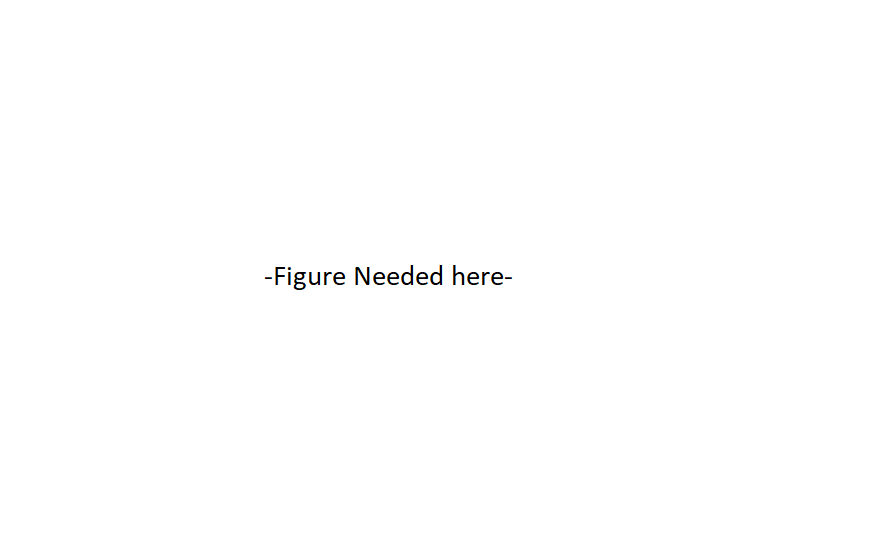
\includegraphics[width=\textwidth]{Figures/Placeholder.png}
	\caption{An example of a planning AI's approach}
	\label{transitions}
\end{figure}
